% Copyright 2020-2022 Robert Bosch GmbH

% Licensed under the Apache License, Version 2.0 (the "License");
% you may not use this file except in compliance with the License.
% You may obtain a copy of the License at

% http://www.apache.org/licenses/LICENSE-2.0

% Unless required by applicable law or agreed to in writing, software
% distributed under the License is distributed on an "AS IS" BASIS,
% WITHOUT WARRANTIES OR CONDITIONS OF ANY KIND, either express or implied.
% See the License for the specific language governing permissions and
% limitations under the License.

\pkg\ is a command-line tool that enables you to import \rfwcore\ XML result 
files into TestResultWebApp's database for presenting an overview about the 
whole test execution and details of each test result.

\begin{figure}[h!]
   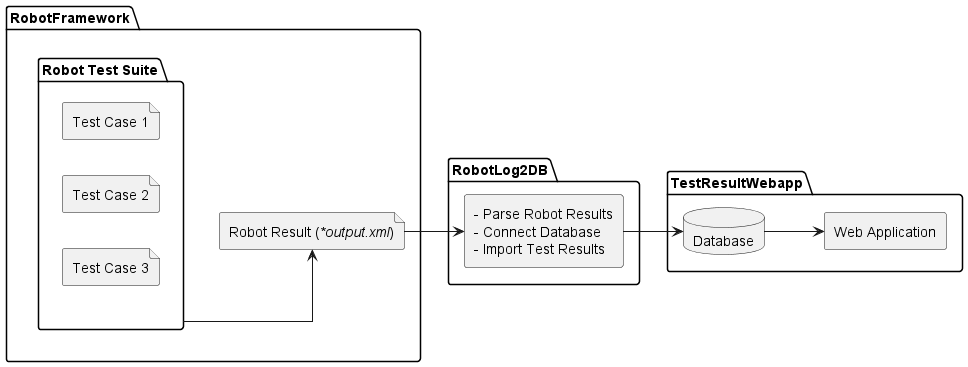
\includegraphics[width=1\linewidth]{./pictures/data_flow.png}
   \caption{Tool data flow}
\end{figure}

\pkg\ tool requires serveral arguments, including the location of the
\href{https://robotframework.org/robotframework/latest/RobotFrameworkUserGuide.html#output-file}
{\rfwcore\ XML result file(s)} to parse all information of test execution result 
and TestResultWebApp's database credential for importing that result.

\href{https://github.com/test-fullautomation/testresultwebapp}{TestResultWebApp} 
requires some mandatory information to manage and display the test result properly. 
Therefore, they should be provided in \rfwcore\ test case before execution, then 
they will be available in XML result file for importing.

However, you can use optional arguments of \pkg\ tool to provide those data 
if they are missing or you want to overwrite them with the expected values.

Finally, \pkg\ also allows you to append existing results in the database, which 
is helpful when you need to update previous test results or add the missing 
XML result file(s) from previous tool execution.
